\documentclass[12pt,reqno]{article}
\usepackage{amsthm, amsmath, amsfonts, amssymb, amscd, mathtools, youngtab, euscript, mathrsfs, verbatim, enumerate, multicol, multirow, bbding, color, babel, esint, geometry, tikz, tikz-cd, tikz-3dplot, array, enumitem, hyperref, thm-restate, thmtools, datetime, graphicx, tensor, braket, slashed, standalone, pgfplots, ytableau, subfigure, wrapfig, dsfont, setspace, wasysym, pifont, float, rotating, adjustbox, pict2e,array}
\usepackage{amsmath}
\usepackage[utf8]{inputenc}
\usetikzlibrary{arrows, positioning, decorations.pathmorphing, decorations.pathreplacing, decorations.markings, matrix, patterns}
\tikzset{big arrow/.style={
    decoration={markings,mark=at position 1 with {\arrow[scale=1.5,#1]{>}}},
    postaction={decorate},
    shorten >=0.4pt},
  big arrow/.default=black}

\begin{document}

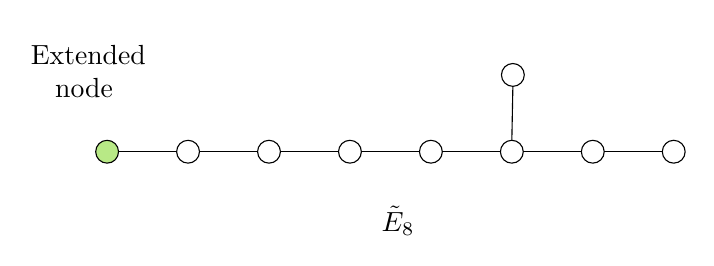
\begin{tikzpicture}[x=0.75pt,y=0.75pt,yscale=-1,xscale=1]

\draw   (455.5,69.5) .. controls (455.5,66.46) and (457.96,64) .. (461,64) .. controls (464.04,64) and (466.5,66.46) .. (466.5,69.5) .. controls (466.5,72.54) and (464.04,75) .. (461,75) .. controls (457.96,75) and (455.5,72.54) .. (455.5,69.5) -- cycle ;
\draw   (416.5,69.5) .. controls (416.5,66.46) and (418.96,64) .. (422,64) .. controls (425.04,64) and (427.5,66.46) .. (427.5,69.5) .. controls (427.5,72.54) and (425.04,75) .. (422,75) .. controls (418.96,75) and (416.5,72.54) .. (416.5,69.5) -- cycle ;
\draw    (427.5,69.5) -- (455.5,69.5) ;
\draw   (377.5,69.5) .. controls (377.5,66.46) and (379.96,64) .. (383,64) .. controls (386.04,64) and (388.5,66.46) .. (388.5,69.5) .. controls (388.5,72.54) and (386.04,75) .. (383,75) .. controls (379.96,75) and (377.5,72.54) .. (377.5,69.5) -- cycle ;
\draw   (338.5,69.5) .. controls (338.5,66.46) and (340.96,64) .. (344,64) .. controls (347.04,64) and (349.5,66.46) .. (349.5,69.5) .. controls (349.5,72.54) and (347.04,75) .. (344,75) .. controls (340.96,75) and (338.5,72.54) .. (338.5,69.5) -- cycle ;
\draw    (349.5,69.5) -- (377.5,69.5) ;
\draw    (388.5,69.5) -- (416.5,69.5) ;
\draw   (299.5,69.5) .. controls (299.5,66.46) and (301.96,64) .. (305,64) .. controls (308.04,64) and (310.5,66.46) .. (310.5,69.5) .. controls (310.5,72.54) and (308.04,75) .. (305,75) .. controls (301.96,75) and (299.5,72.54) .. (299.5,69.5) -- cycle ;
\draw   (260.5,69.5) .. controls (260.5,66.46) and (262.96,64) .. (266,64) .. controls (269.04,64) and (271.5,66.46) .. (271.5,69.5) .. controls (271.5,72.54) and (269.04,75) .. (266,75) .. controls (262.96,75) and (260.5,72.54) .. (260.5,69.5) -- cycle ;
\draw    (271.5,69.5) -- (299.5,69.5) ;
\draw   (221.5,69.5) .. controls (221.5,66.46) and (223.96,64) .. (227,64) .. controls (230.04,64) and (232.5,66.46) .. (232.5,69.5) .. controls (232.5,72.54) and (230.04,75) .. (227,75) .. controls (223.96,75) and (221.5,72.54) .. (221.5,69.5) -- cycle ;
\draw  [fill={rgb, 255:red, 184; green, 233; blue, 134 }  ,fill opacity=1 ] (182.5,69.5) .. controls (182.5,66.46) and (184.96,64) .. (188,64) .. controls (191.04,64) and (193.5,66.46) .. (193.5,69.5) .. controls (193.5,72.54) and (191.04,75) .. (188,75) .. controls (184.96,75) and (182.5,72.54) .. (182.5,69.5) -- cycle ;
\draw    (193.5,69.5) -- (221.5,69.5) ;
\draw    (232.5,69.5) -- (260.5,69.5) ;
\draw    (310.5,69.5) -- (338.5,69.5) ;
\draw    (383.5,38) -- (383,64) ;
\draw   (378,32.5) .. controls (378,29.46) and (380.46,27) .. (383.5,27) .. controls (386.54,27) and (389,29.46) .. (389,32.5) .. controls (389,35.54) and (386.54,38) .. (383.5,38) .. controls (380.46,38) and (378,35.54) .. (378,32.5) -- cycle ;

% Text Node
\draw (319,94.4) node [anchor=north west][inner sep=0.75pt]    {$\tilde{E}_{8}$};
% Text Node
\draw (150,10) node [anchor=north west][inner sep=0.75pt]   [align=left] {\begin{minipage}[lt]{38.44pt}\setlength\topsep{0pt}
\begin{center}
Extended \\node
\end{center}

\end{minipage}};


\end{tikzpicture}

\end{document}